%\clearpage{\pagestyle{empty}\cleardoublepage}

%\chapter{Object reconstruction}\label{chap:objects}
\section{Object reconstruction}\label{sec:objects}

After having described the ATLAS detector, in the following Section we will
explain how object (electrons, muons, jets and the missing transverse energy \met) 
are reconstructed to be used in physics analyses~\cite{Aad:2009wy}. Details from
selections specific for the analyses presented in this dissertation are given.


%\section{Electrons}\label{sec:electrons}
\subsection{Electrons}\label{sec:electrons}
Electrons~\cite{eperf} are reconstructed for pseudorapidities up to $|\eta| = 2.5$, where
information from the ID is available, matching a track with an energy deposit
(cluster) in the electromagnetic calorimeter. 

To identify tracks from ID points an inside-out algorithm is used, starting from a 
seed of three aligned hits in the pixel detector or in the SCT. Five fundamental parameters,
shown and described in Figure~\ref{fig:trackpar}, are computed and used for the subsequent 
steps of hits association. The candidate track must be formed by at least seven points
measured in the silicon detectors, $d_0$ must be lower than 10~mm and the 
transverse momentum must be higher than 150~\mev.

\begin{figure}[tb]\begin{center}
	\subfigure[]{
  	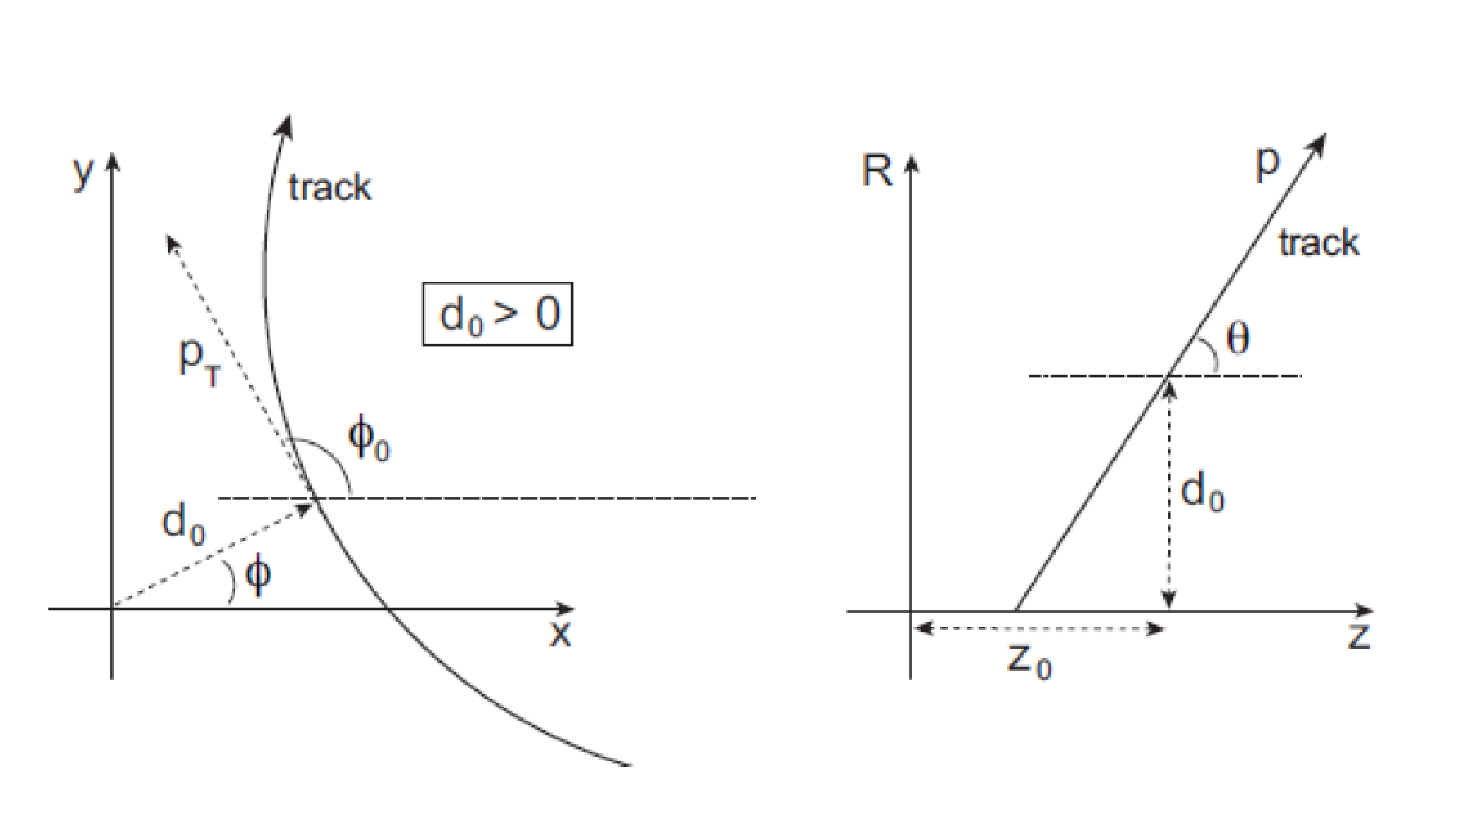
\includegraphics[width=0.7\textwidth]{objectsreconstruction/figures/tracks}}
	\caption[bla]{Schematic drawings of the parameters used for track reconstruction in the XY and $R$Z planes (left and right respectively)
          where the origin is the reconstructed primary vertex\footnotemark.
          The parameters are: $q/p$, the charge divided by the momentum; $\theta$, or more used $\eta$, the angle
          with respect to the Z axis in the $R$Z plane measured from the perigee; $\phi_0$, the angle 
          with respect to the X axis in the XY plane measured from the perigee; $d_0$, the impact parameter, 
          or perigee with respect to the Z axis in the XY plane; $z_0$, Z component of the perigee.\label{fig:trackpar}}
\end{center}\end{figure}

\footnotetext{Of the reconstructed verteces consistently in the beam collision region in the XY plane with at least five associated tracks, the one with the highest number of tracks is taken as the primary one.}
Clusters~\cite{topocluster} are built starting from
$\Delta\eta\times\Delta\phi=0.025\times0.025$ single energy deposits summing
up into towers. Adjacent towers form clusters of $3\times7$ cells units in $\eta\times\phi$
in $|\eta|<1.4$ and $5\times5$ further. Of all the candidate reconstructed tracks,
those extrapolated to the calorimeter with the smallest $\dr$ with respect to the
energy cluster is chosen.

For our analyses, electrons in the transition region $1.37<|\eta_{\rm cluster}| <1.52$
with inactive material are excluded. Electrons are also required to have 
$\et = E_{\rm cluster}/\cosh\eta_{\rm track} > 25\gev$ and $z_0<2~$mm.
They have to be separated from any jet (Section~\ref{sec:jets}) selected by at least $\dr =0.4$.
90\% efficient isolation cuts to reduce the background from non-prompt electrons coming from
hadron decays are defined, one based on the energy from calorimeter cells surrounding the candidate in
a cone of radius $R=0.2$ and the other based on the track transverse momenta sum in a cone of radius $R=0.3$ around
the electron.

%\section{Muons}\label{sec:muons}
\subsection{Muons}\label{sec:muons}
Track segments reconstructed in the muon spectrometer are matched to tracks from the ID to build
muon candidates. The combined tracking information has to give $p_T>25\gev$ and $|\eta|<2.5$, and
$z_{0}$ has to be lower than 2~mm.
The muon radial distance from any selected jet is required to be $\Delta R > 0.4$.

A  $\pt$-dependent track-based isolation condition is defined as follows:
the scalar $\pt$ sum of all tracks (except for the muon track itself) 
in a cone of variable radius $R=10\gev/\pt^\mu$ around the lepton
must be less than 5\% of the muon $\pt$.
This isolation requirement works well also in high pile-up events
or in the case the muon is close to a jet.

%\section{Jets}\label{sec:jets}
\subsection{Jets}\label{sec:jets}

Jets from quark hadronization are reconstructed using the anti-$k_t$
algorithm~\cite{ref:Cacciari2008,ref:Cacciari2006,ref:fastjet} with a
radius parameter $R=0.4$ (from which the algorithm is often referred to as anti-$k_t$4) 
using calorimeter energy deposits\footnote{Topological clusters, abbreviated as ``topo-clusters'', are 
built from neighboring calorimeter cells starting from a seed deposit with a signal to noise ratio
higher than a certain threshold. Topo-clusters are treated as massless and their energy at the electromagnatic 
scale is the sum of the constituent cells.}
corrected for effects of non-compensation,
dead detector material and out-of-cluster leakage using local cluster calibrations~\cite{LCW1,LCW2}.

To subtract contributions from in-time and out-of-time pile-up interactions a correction is applied
parameterized according to the number of primary vertices in the event and the number of average interactions 
in the luminosity block ($<\mu>$) as a function of jet pseudorapidity.
Jets are finally calibrated to the hadronic scale using $\pt$- and $\eta$-dependent correction factors 
derived from Monte Carlo simulation~\cite{jes}.
For the analyses that we will present, only jets with $\pt > 25\gev$ and $|\eta| < 2.5$ are considered.

A variable called ``jet vertex fraction" (JVF) is defined as the fraction
of the sum of $\pt$ of tracks with $\pt>1\gev$
associated with the jet that comes from tracks originating from the primary vertex.
By requiring JVF$>0.5$ we avoid selecting jets from in-time pile-up events.

Since energy deposits from electrons can be reconstructed as jets, 
if jets are found within $\Delta R$ of 0.2 of a selected electron, the
jet closest to the lepton is discarded in order to avoid double-counting of electrons as jets.
After this one jet has been removed, electrons that lie within $\Delta R< 0.4$ of 
the jets remaining are removed.

A technique to identify jets from the hadronisation of bottom quarks, 
called $b$-tagging~\cite{ref:ATLAS-CONF-2011-102}, is used. It
makes use of multivariate techniques combining the information
from secondary and tertiary decay vertices found within the jet
and from the impact parameters of displaced tracks to obtain a 
$b$-tagging weight that discriminates between $b$ and not-$b$
jets. A working point for this weight is chosen by finding
a compromize between a good efficiency (the ratio between tagged 
$b$-jets and true $b$-jets) and a high light-jet rejection
(the inverse of the number of light-jets misidentified as $b$-jets).
For our analyses, a working point corresponding to  70\% efficiency, 
$\sim$130 light-jet rejection and a charm-jet rejection of 5 is 
chosen\footnote{These values refer to jets with $\pt >20\gev$ and 
$|\eta|<2.5$ in simulated $t\bar{t}$ events.}


%\section{Missing Transverse Energy}\label{sec:met}
\subsection{Missing transverse energy}\label{sec:met}

To estimate the momentum of invisible particles in the event,
the missing transverse energy $\met$~\cite{met} is defined by first matching each calorimeter energy 
deposit with a high-$\pt$ lepton or jet. After the energies of these objects are
corrected accordingly to the respective calibration constants, the calorimeter clusters
that did not get associated with any  high-$\pt$ object are calibrated for energy losses in 
dead material regions and for the different response to the electromagnetic and hadronic
components of particle showers. Finally the \met\ is computed from the combinetion of the vector 
sum of the calibrated cluster momenta and a term associated with muon momenta.
